\documentclass[a4paper,11pt]{resume}
\usepackage[utf8]{inputenc}
\usepackage{graphicx}
\usepackage{amsmath}
\usepackage{float}
\usepackage[left=0.75in,top=0.75in,right=0.75in,bottom=0.7in]{geometry}
\usepackage{titling}
\usepackage{hyperref}
\newcommand{\subtitle}[1]{%
  \posttitle{%
    \par\end{center}
    \begin{center}\large#1\end{center}
    \vskip0.5em}%
}
\usepackage{atbegshi}
\AtBeginDocument{\AtBeginShipoutNext{\AtBeginShipoutDiscard}}
\usepackage{etoolbox}
\patchcmd{\thebibliography}{\section*{\refname}}{}{}{}

\title{Learning to play Tetris with Big Data: Project Report}
\subtitle{CS 3243 - Introduction to Artificial Intelligence (Group 14)}
\author{\bf{Yogesh Kumar} \\ A0149495M  
\and \bf{Narinderpal Singh} \and \bf{Nhan Nguyen} \and \bf{Kristoffer Pederson} \\ E0013699 \and \bf{Gustav Kvick} \\ E0009428
    }
\date{\today}

\begin{document}
\vspace{-15pt}
\maketitle
\vspace{-5pt}
\begin{rSection}{{\heading Introduction}}
\begin{rSubsection}{}{}{}{}
\vspace{-5pt}
\item The purpose of the project is to create a utility based agent whose goal is to maximize the number of rows removed up to termination of the game. 


\begin{minipage}{0.65\textwidth}
\item Tetris is a video game which was originally invented by Russian programmer Alex Pajitonv at 1985. Then It has been popular since the day. The blocks, usually called Tetrominos, fall from the top of the board to the bottom.
\end{minipage}
\begin{minipage}{0.30\textwidth}
\centering
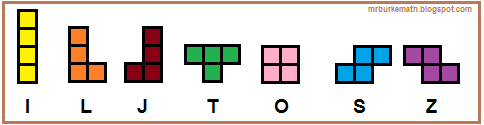
\includegraphics[width=\textwidth,scale=0.4]{tet.png}
\label{fig:find}
\caption{Fig 1: Tetrominos}
\end{minipage}
\\ 
\item The agent uses a heuristic function to approximate the utility of a state. The agent's strategy to play Tetris is improved after every move using the Least Squares Policy Iteration Algorithm.

\item In this report we have given a gist of our design, its salient features and working.
\end{rSubsection}
\end{rSection}

\begin{rSection}{{\heading Strategy of the Agent}}
\begin{rSubsection}{}{}{}{}
\vspace{-5pt}
\item 
Given the current piece to place, the agent will choose the decision that will give the best board. When a piece is to be placed, the agent simulates and evaluates all the possible boards that would result from all the possible moves(orientations and positions) of the piece, and then chooses the action that leads to the best valued game board (greedy strategy).

\item We note $s \in S$ a state of the game, $s$ represents the configuration of the board at a given time. The evaluation function $V : S \to \rm I\!R}$ maps a state $s$ to a number that estimates the value of the state $s$.

\item The evaluation function $V$ is a combination of the feature functions using generally a weighted linear sum. If we let $f_i$ and $w_i$, with $i = 1...n$, denote the n feature functions and their respective weights. Each $f_i$ maps a state $s$ to a real value. The evaluation function $V$ is then defined as:
\end{rSubsection}
\end{rSection}
\vspace{-20pt}
\begin{align}
  \  V(s)=\sum_{i=1}^{n} w_if_i(s)
\end{align}
\begin{rSection}{{\heading Feature functions}}
\begin{rSubsection}{}{}{}{}
\vspace{-5pt}
\item The following features are evaluated in the heuristic function.
\vspace{-5pt}
\begin{enumerate}
    \item {\bf{Landing height}}: the height at which the current piece fell
    \vspace{-5pt}
    \item {\bf{Eroded pieces}}: the contribution of last piece to the cleared rows time the no. of cleared rows
    \vspace{-20pt}
    \item {\bf{Row transitions}}: number of filled cells adjacent to empty cells summed over all rows
    \vspace{-5pt}
    \item {\bf{Column transitions}}: number of filled cells adjacent to empty cells summed over all columns
    \vspace{-5pt}
    \item {\bf{Number of holes}}: the number of empty cells with at least one filled cell above
    \vspace{-5pt}
    \item {\bf{Cumulative wells}}: the sum of the accumulated depths of the wells
    \vspace{-5pt}
    \item {\bf{Hole depth}}: the number of filled cells above holes summed over all columns
    \vspace{-5pt}
    \item {\bf{Row hole}}: the number of rows that contains at least one hole
\end{enumerate}
\centering
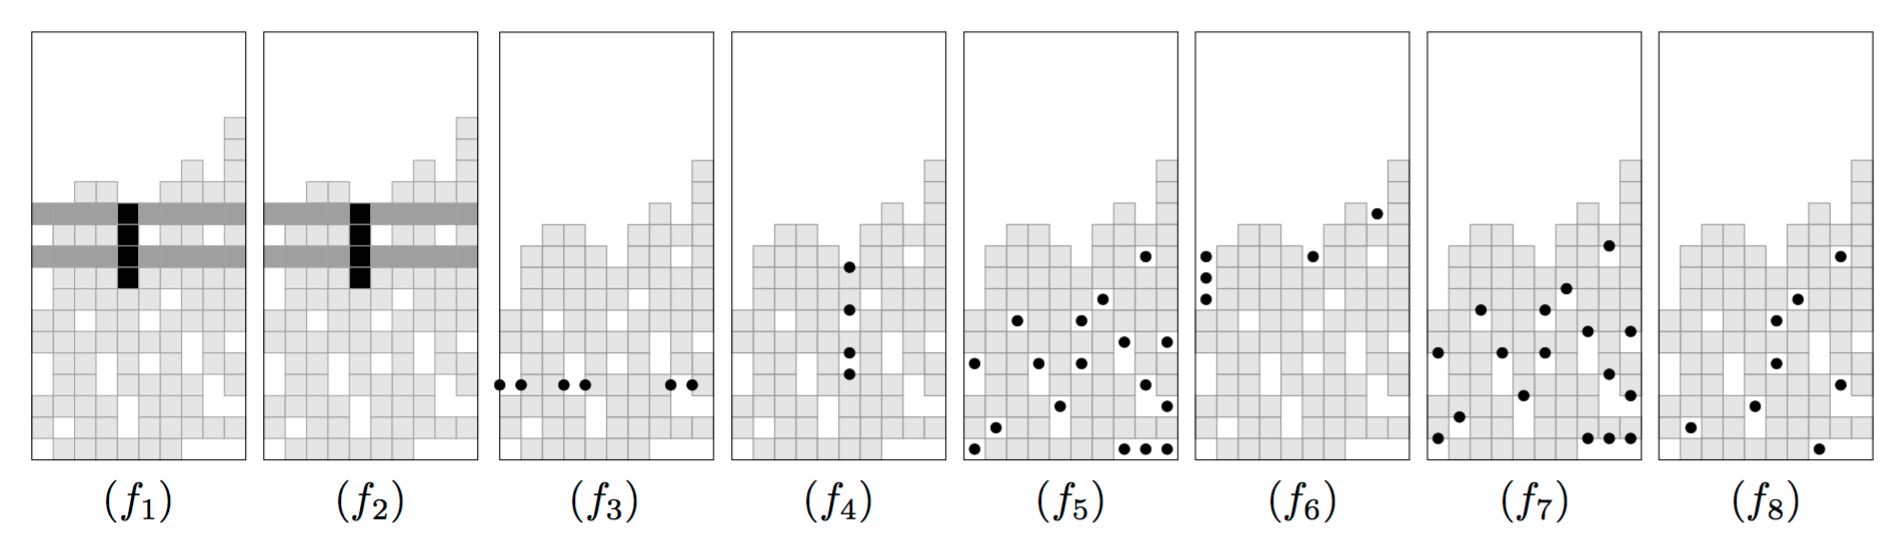
\includegraphics[width=\textwidth,scale=0.4]{features.png}
\label{fig:find}
\caption{Figure 2: Features functions}
\end{rSubsection}
\end{rSection}

\end{document}